\section{Protolys}

Protolys\footnote{se s. 60 i boken}---från \emph{proto} för proton och forngrekiskans \emph{lúsis} för lossa---innebär att det sker ett utbyte av en eller flera protoner ($\ce{H+}$ joner). Som angivet ovan kommer syror lossa en proton och baser ta emot en.
\begin{exm}
    Låt en syra A som innehåller en väteatemom H reagera med vatten. Detta kallas också att den \emph{protolyseras}:
    \begin{center}
        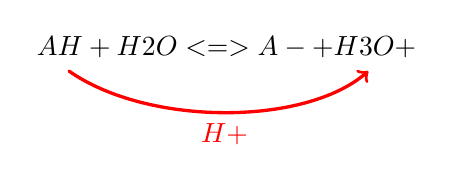
\begin{tikzpicture}
            \node at (0,0) {$\ce{AH + H2O <=> A- + H3O+}$};
            \draw[very thick, color=red, ->, line cap=round] (-2,-0.3) .. controls (-1,-1) and (1,-1) .. node[anchor=north] {$\ce{H+}$} (1.8,-0.3);
        \end{tikzpicture}
    \end{center}
    Något mycket liknande sker när en bas B protolyseras:
    \begin{center}
        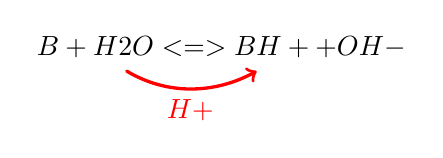
\begin{tikzpicture}
            \node at (0,0) {$\ce{B + H2O <=> BH+ + OH-}$};
            \draw[very thick, color=red, ->, line cap=round] (-1.2,-0.3) .. controls (-0.7,-0.6) and (-0.1,-0.6) .. node[anchor=north] {$\ce{H+}$} (0.45,-0.3);
        \end{tikzpicture}
    \end{center}
\end{exm}

\subsection{Svaga/starka syror och baser}
Man säger att en syra eller en bas kan antingen vara stark eller svag\footnote{se s. 63 samt uppgift 3:29--3.20 i boken}. Detta har faktiskt ingen korrelation med hur mycket den förändrar pH utan det betecknar om reaktionen är fullständig. En syra/bas som protolyseras helt när den placeras i vattelösning kallas stark och alla andra är svaga.

\section{pH och pOH}

Dessa är ett mått på hur syrligt eller basiskt en lösning är. pH är absolut standard med det finns anvädningar för pOH också. Skalan är logaritmisk med bas 10 och går från ca -1 till ca 14. Definitionen för de två storheterna är:
\begin{align*}
    \mathrm{pH} &= -\log_{10}{\ce{[H3O+]}} \\
    \mathrm{pOH} &= -\log_{10}{\ce{[OH^-]}}
\end{align*}
Ju högre pH är desto mer basiskt och ju mer basiskt desto mindre desto mer syrligt. En neutral lösning har pH 7. Då är $\ce{[H3O+] = [OH^-]}$. För att beräkna ena eller andra vet vi även detta samband:
\[
    \mathrm{pH + pOH} = 14
\]

\section{Syra- och baskonstanten}

Mycket likt jämviktskonstanten $K$ finns den en så kallad \emph{syrakonstant} $K_a$ och en \emph{baskonstant} $K_b$. Dessa beskriver hur fullständig en syra/bas protolyseras. Dessa värde existerar även för amfolyter---ämnen som är både syra och bas---och bestämmer då om de hellre reagerar som syra eller bas. Dessa värde är som $K$ för för protolysen men man bortser från [$\ce{H2O}$] alltså ser det ut som:
\begin{align*}
    K &= \frac{\mathrm{[Bas]} \cdot [\ce{H3O+}]}{\cancel{\ce{[H2O]}} \cdot \mathrm{[Syra]}} \\
    K_a &= \frac{\mathrm{[Bas]} \cdot [\ce{H3O+}]}{\mathrm{[Syra]}} 
\end{align*}
för en syra och följande för en bas:\begin{align*}
    K &= \frac{\mathrm{[Syra]} \cdot [\ce{OH^-}]}{\cancel{\ce{[H2O]}} \cdot \mathrm{[Bas]}} \\
    K_b&= \frac{\mathrm{[Syra]} \cdot [\ce{OH^-}]}{\mathrm{[Bas]}} 
\end{align*}

\subsection{Räkna med syra- och baskonstanten}
Man räknar på dessa konstanter ungefär som man räknar med $K$ (se \vref{sec:räknak}). Skillnaden är att du kommer veta $K_a \text{ eller } K_b$ i förväg från en tabell. Du kan sedan utnyttja detta för att ställa upp jämvikten med tidigare angivna tabeller för att sedan beräkna $\ce{[H3O+] \text{ eller } [OH^-]}$ i en lösning som i sin tur kan leda till pH. 